\chapter{METODOLOGIAS E FERRAMENTAS}
\label{cap:elementos}

Para o desenvolvimento dos projetos são utilizadas metodologias ágeis de desenvolvimento e ferramentas para desenvolvimento web (backend e frontend). Para entender melhor essas tecnologias as seções seguintes aborda cada uma delas.
\section{Metodologias Ágeis}

\begin{quote}
  O "Manifesto ágil" surgiu em 2001 quando 17 conhecedores de metodologias ágeis se reuniram e discutiram como deveria ser o processo de desenvolvimento de software com metodologias ágeis, elencando 12 princípios que priorizam principalmente a satisfação do cliente, o trabalho em equipe, entregas de software mais rápidas e colaboração com o cliente. - \cite{manifestoAgil}
\end{quote}

São estratégias e comportamentos que devem ser seguidos afim de obter um resultado otimizado e mensurável.

\subsection{Scrum}

Metodologia ágil que visa ter escopo fechado (número de tarefas predefinidas), calculadas através de métricas da equipe, como pontos de esforço.

Foi desenvolvida baseada nas metodologias de empresas do japão, como Toyota e Honda. É um framework de trabalho que pode ser adaptado para diversas áreas.

As tarefas a serem desenvolvidas ficar armazenadas no product backlog, sendo retiradas de la as com maior prioridades para serem inseridas na sprint.

Também existem alguns ritos que devem ser seguidos para o bom funcionamento do Scrum, como as Daily Meetings, Planning, Review Meeting e Retrospective, que ocorrem em um fluxo como descrito na Figura \ref{fig:scrum}.

\begin{figure}[H]
\centering
\caption{Fluxo Scrum} %legenda
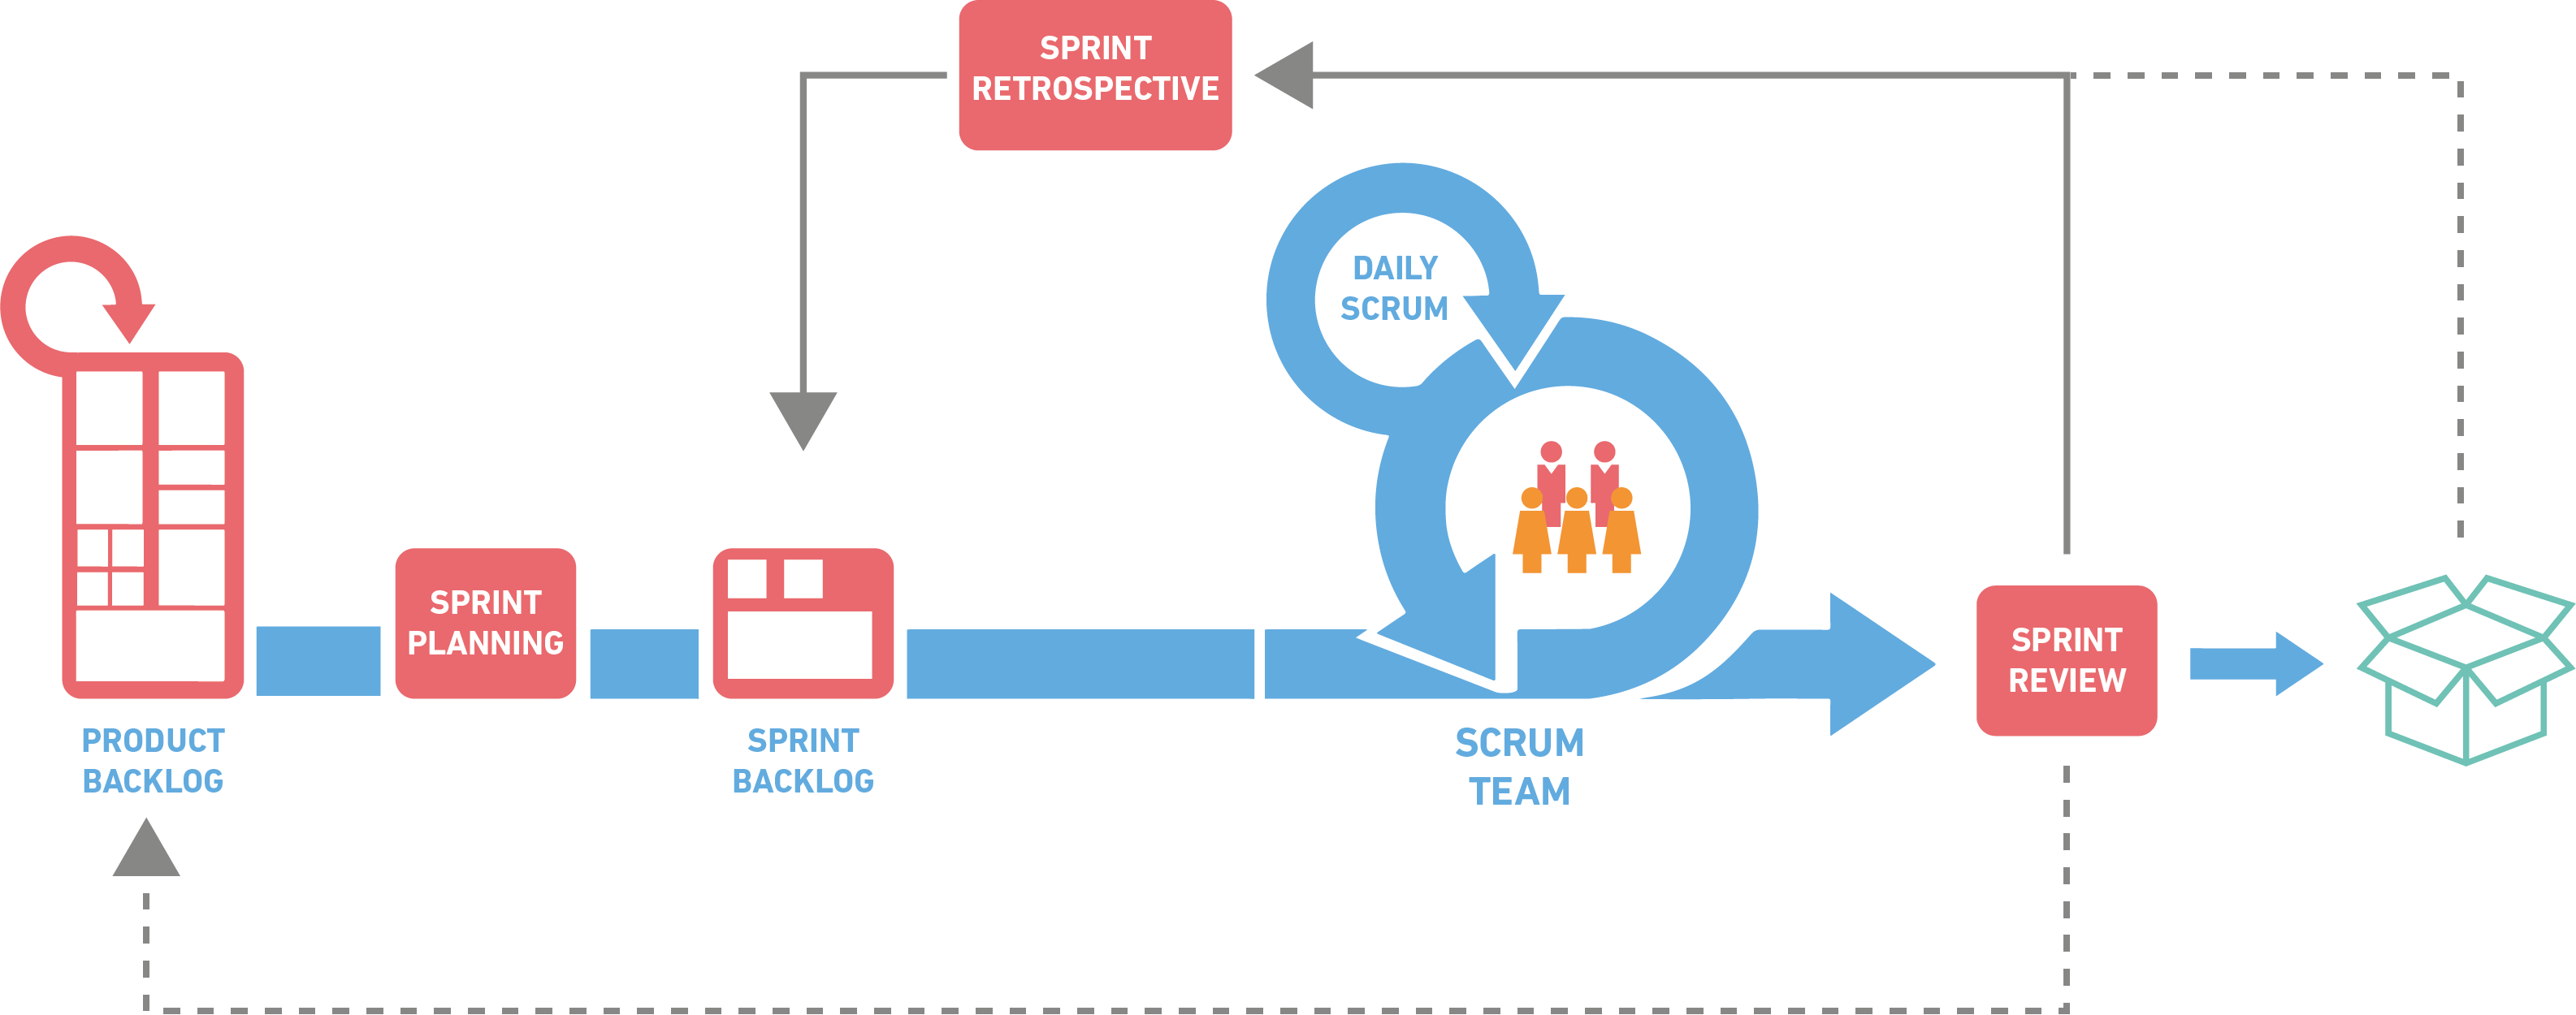
\includegraphics[scale=0.2]{Scrum}\\  % o 0.9 indica 90% do tamanho original
% pdfLaTeX aceita figuras no formato PNG, JPG ou PDF
% figuras vetoriais podem ser exportadas para eps e depois convertidas para pdf usando epstopdf
{\small Fonte:https://blog.mjv.com.br/frameworks-ágeis-saiba-como-funcionam-na-pratica} %Fonte da imagem
\label{fig:scrum} %rotulo para refencia
\end{figure}

Daily Meetings são reuniões diarias, rapidas e praticas para atualização da equipe sobre no que cada um está trabalhando, para um melhor entendimento da equipe.

Review Meetings são reuniões feitas após o fim de cada Sprint, para entender os resultados da equipe durante a sprint.

Retrospective é uma reunião que ocorre todo fim de sprint para identificar o que funcionou e o que pode ser melhorado na sprint.

Planning é a reunião que deve ser feita antes de cada Sprint para definir quais atividades devem ser desenvolvidas, entender melhor sobre elas, descrevendo-as minuciosamente e prevendo possíveis problemas.
Quem gerencia esse product backlog é o  ~\nameref{sec:po}, que cuida de organizar, definir e priorizar as tarefas.

Muitas vezes separadas em Sprints (tempo pré-definido pela equipe, geralmente de 10 dias úteis), as tarefas são incluídas em um quadro e devem ser finalizadas no prazo previsto.

\begin{quote}
  Scrum é um framework simples e pequeno e, assim, funciona bem em  cada contexto se for utilizado em conjunto com outras técnicas e praticas a serem experimentadas e adaptadas. - \cite{sabbagh2014scrum}
\end{quote}
\begin{quote}
  O sprint é o ciclo de desenvolvimento, onde o incremento do produto pronto é gerado pelo Time de Desenvolvimento a partir dos itens mais importantes do Product Backlog. - \cite{sabbagh2014scrum}
\end{quote}


\subsubsection{Scrum Master}

Cargo que tem como função cuidar das obrigações impostas sobre a metodologia scrum, como lembrar dos ritos, marcar reuniões e garantir o bom desenvolvimento das atividades estabelecidas para a sprint.

\begin{quote}
Garante que o time esteja
totalmente funcional e
produtivo.

Facilita a colaboração entre as
funções e áreas e elimina os
impedimentos do time.

Protege o time de
interferências externas.

Garante que o processo está
sendo seguindo. Participando
das reuniões diárias, revisão
da Sprint, e planejamento. \cite{sabbagh2014scrum}

\end{quote}

\subsubsection{Analista de Qualidade(Tester)}

Responsável por encontrar problemas e possíveis melhorias durante o desenvolvimento, garantido o funcionamento total do sistema para que seja validado com o cliente.

\subsubsection{Gerente de projetos(GP)}

Cargo que tem como função gerenciar os projetos e times da sua
 tribo, cuidando para que sejam entregues os requisitos no prazo combinado.

\begin{quote}
  O gerente de projetos é a pessoa destacada e designada como principal responsável por atingir os objetivos do projeto. - \cite{cruz2013scrum}
\end{quote}
\subsubsection{Product Owner(PO)}
\label{sec:po}
Cargo que tem como função cuidar do relacionamento do time com o produto,
 definindo e priorizando requisitos.
 
 \begin{quote}
  Define os requisitos do
  produto, decide a data de
  release e o que deve conter
  nela.

  É responsável pelo retorno
  financeiro (ROI) do produto.
  
  Prioriza os requisitos de
  acordo com o seu valor de
  mercado.
  
  Pode mudar os requisitos e
  prioridades a cada Sprint.
  o Aceita ou rejeita o resultado de
  cada Sprint. - \cite{sabbagh2014scrum}
 \end{quote}

\subsection{Kanban}
Opção de metodologia ágil mais adaptativa, tendo escopo aberto torna-se possível inserir atividades durante o tempo.
Muitas vezes é comparado a uma tubulação de agua, onde existe uma determinada quantidade de agua a ser transportada, porem é necessário definir o tamanho do tubo ou vazão, sendo esse, a quantidade de esforço que a equipe consegue trabalhar.
Assim como o Scrum, possui um backlog controlado por um Product Owner. As atividades são inseridas assim que libera oque chamamos de vazão, como em uma tubulação.
Diferentemente do Scrum, não há necessidade de Reviews e Retrospective uma vez que não possui sprints, porem algumas reuniões para analisar o desempenho da equipe são um boa pratica.
Geralmente é determinado um máximo de esforço e, ao final de uma atividade, é inserida uma nova com prioridade.


  \begin{quote}
    O kanban, ou mais precisamente o "sistema Kanban para desenvolvimento de software" representa uma implementação mais direta dos princípios de Desenvolvimento Lean de Produtos para o desenvolvimento de software que os métodos aágeis tradicionais. Com foco consistente no fluxo e no contexto, o Kanban oferece uma abordagem menos prescritiva comparada ao Agile, e tem se tornado uma extensão popular dos métodos ágeis tradicionais como Scrum e XP. - \cite{boeg2010kanban}
  \end{quote}
\begin{figure}[H]
\centering
\caption{Quadro kanban} %legenda
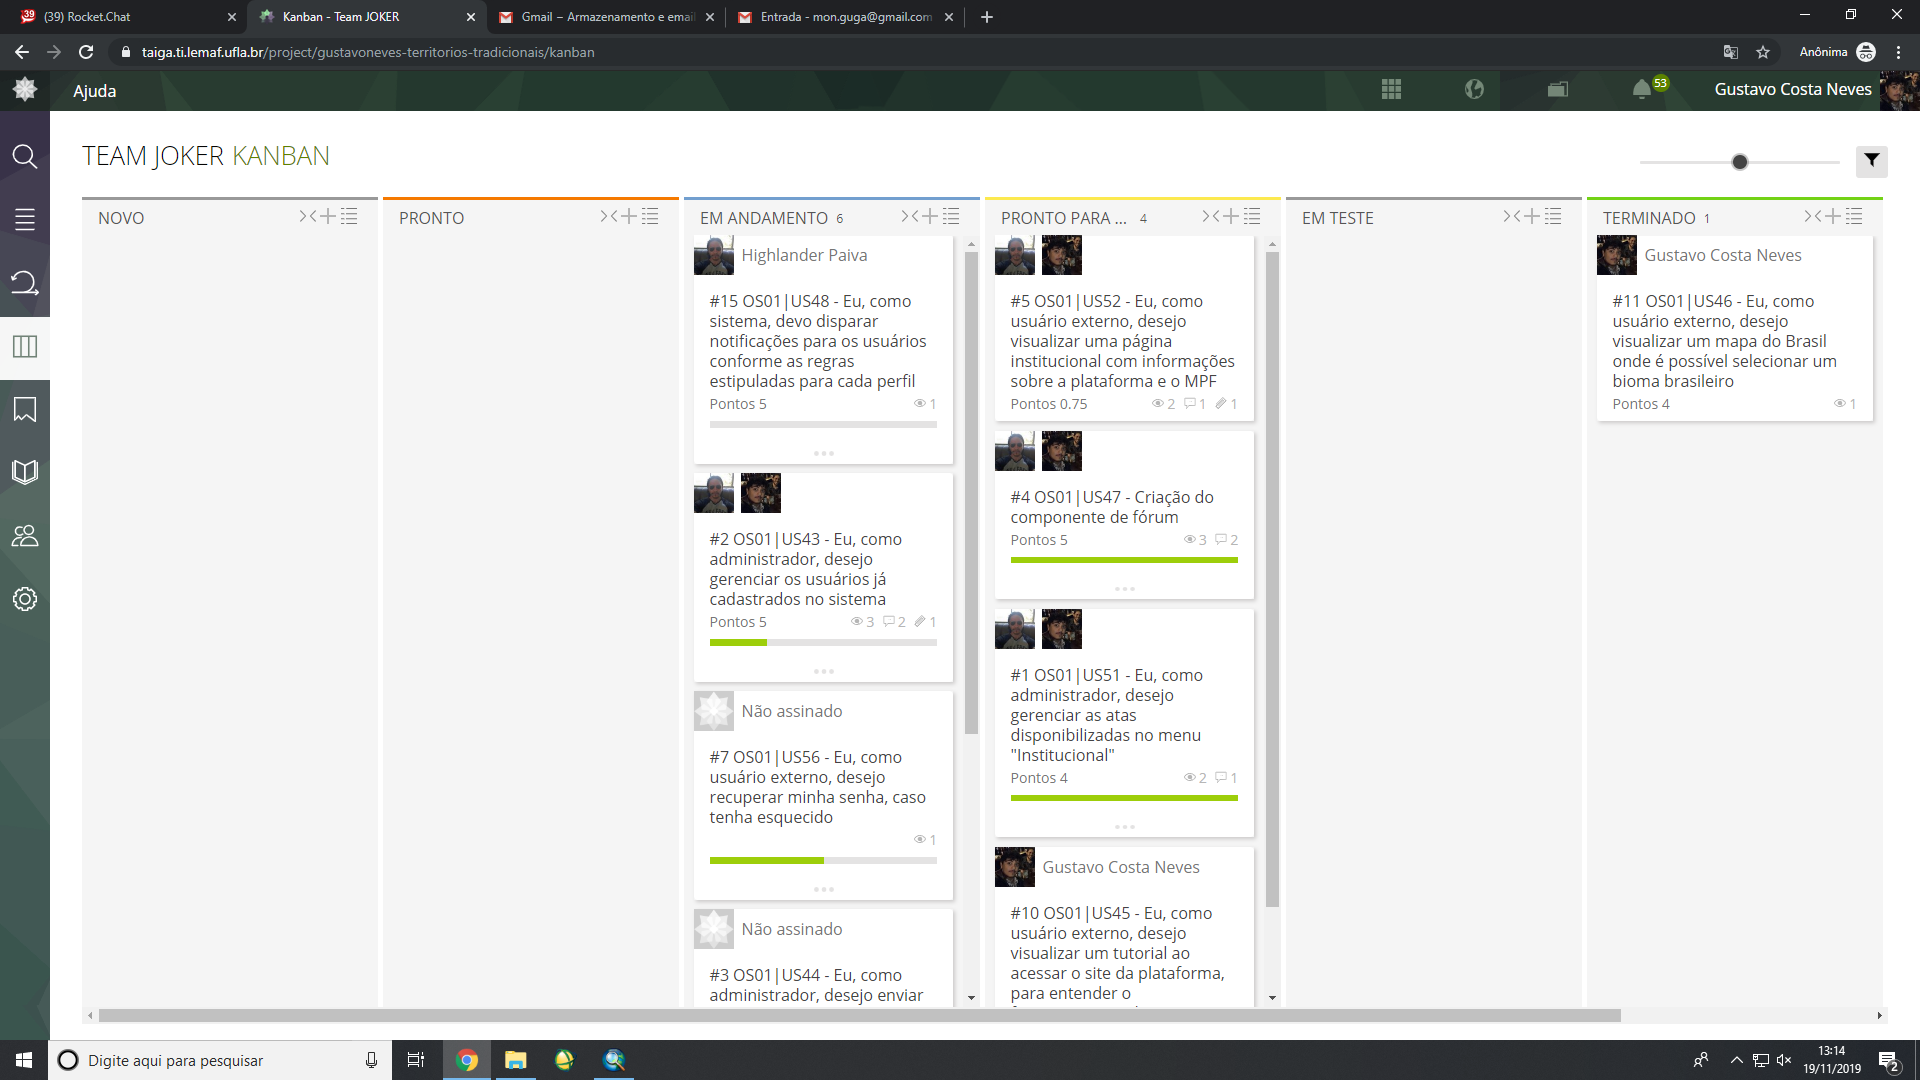
\includegraphics[scale=0.2]{quadroKanban}\\  % o 0.9 indica 90% do tamanho original
% pdfLaTeX aceita figuras no formato PNG, JPG ou PDF
% figuras vetoriais podem ser exportadas para eps e depois convertidas para pdf usando epstopdf
{\small Fonte: https://taiga.ti.LEMAF.ufla.br/} %Fonte da imagem
\label{fig:exemplo} %rotulo para refencia
\end{figure}

\section{Frameworks}

Para facilitar o desenvolvimento, diversas ferramentas foram criadas e durante o desenvolvimento de novos projetos foi necessária a utilização das mesmas.

As aplicações que utilizam esses frameworks geralmente são separadas em frontend e backend. Isto facilita a modularização das aplicações, uma vez que um backend pode ser utilizado por diversos frontend e o contrario também é possível.

\subsection{Frontend}

É a parte da aplicação que interage diretamente com o usuário.

\subsubsection{Angular}

Angular é um framework open-source, de desenvolvimento front-end, que possibilita o desenvolvimento de aplicações web.

Teve sua primeira versão lançada em 2016.

\begin{quote}
  o AngularJS foi criado por Miško Hevery e Adam Abron  em  2009  e  é  um  framework  JavaScript open  source(código  aberto), client-side(do lado  do  cliente)  que  promove  uma  alta  produtividade  na  experiência  do  desenvolvimento Web - \cite{ferreira2018analise}
\end{quote}


\subsubsection{VueJS}

Vue.js é um framework JavaScript de open-source, focado no desenvolvimento de interfaces de usuário e aplicativos de página única.

Teve sua primeira versão lançada em 2014.

\begin{quote}
  Vue é uma lib/framework JavaScript reativo, para  o  desenvolvimento  de  componentes  que,  por  sua  vez,  são  códigos  que  podem  ser reaproveitados em sua aplicação - \cite{ferreira2018analise}
\end{quote}


\subsubsection{ReactJS}

O React é uma biblioteca JavaScript, open-source, com foco em criar interfaces de usuário em páginas web. É mantido por empresas como Facebook e Instagram e uma comunidade de desenvolvedores individuais. 

Teve sua primeira versão lançada em 2013.

\begin{quote}
  Segundo a sua documentação(2018), ele é, na  verdade,  uma  biblioteca  de  UI  (User  Interface),  representando  apenas  a  camada view do Model  View  Controler(MVC).  - \cite{ferreira2018analise}
\end{quote}

\subsection{Backend}

É a parte da aplicação que é inacessível ao usuário, onde é controlado todo o sistema (autenticação, regras de negocio, jobs e etc).

\subsubsection{PlayFramework}

O Play Framework é uma alternativa "limpa" de esticar as stacks do Java Enterprise. Ele se concentra na produtividade do desenvolvedor e tem como objetivo arquiteturas RESTful. 

O objetivo da estrutura do Play é facilitar o desenvolvimento de aplicativos da web, mantendo o Java.

Teve sua primeira versão lançada em 2009.

\begin{quote}
Play! Framework 2 é planejado para ser "full stack" e completamente integrada, a boa notícia é que não há requisitos específicos para você ou seu ambiente começar a criar novos aplicativos da web. - \cite{petrella2013learning}
\end{quote}

\subsubsection{Spring Boot}

O Spring é um framework open-source para a plataforma Java criado por Rod Johnson e descrito em seu livro "Expert One-on-One: JEE Design e Development".
Trata-se de um framework baseado nos padrões de projeto inversão de controle e injeção de dependência.

Teve sua primeira versão em 2002.

\begin{quote}
  Spring Framework é um framework voltado para desenvolvimento de aplicações corporativas para a plataforma Java, baseado nos conceitos de inversão de controle e injeção de dependências. - \cite{weissmann2014vire}
\end{quote}

\subsubsection{DotNet Framework}

O .NET Framework é uma iniciativa da empresa Microsoft, que visa uma plataforma única para desenvolvimento e execução de sistemas e aplicações.
Todo e qualquer código gerado para .NET pode ser executado em qualquer dispositivo que possua um framework de tal plataforma.

Teve sua primeira versão lançada em 2002.

\begin{quote}
  
O .Net Framework é um framework de desenvolvimento que fornece uma nova interface de programação para serviços e APIs do Windows e integra várias tecnologias que surgiram da Microsoft no final dos anos 90. \cite{thai2003net}
\end{quote}

\subsection{Banco de Dados}

É aonde ficam armazenadas informações necessárias para o funcionamento das aplicações.

\subsubsection{Postgresql}

É um sistema gerenciador de banco de dados desenvolvido na linguagem de programação C.
Gerencia banco de dados relacionais e possui ótimo desempenho.

Possui extensões que contribuem com sua eficacia, como por exemplo o POSTGIS, uma extensão que possibilita o Postgresql a utilizar dados Geoespaciais.
Um das vantagens é que sua licença é gratuita desde fins estudantis a empresariais.
Teve sua primeira versão lançada em 2009.

\begin{quote}
  O PostgreSQL é uma das opções de banco de dados, pois se trata de um servidor SGBD de grande potencial e confiabilidade, contendo todas as características dos principais bancos de dados utilizados no mercado. Uma das suas características são suas licenças para uso gratuito, seja para fins estudantis seja para a realização de negócios, possibilitando que empresas o utilizem livremente. \cite{postgres}
\end{quote}